% This work is licensed under the Creative Commons Attribution-NonCommercial 4.0 International License.
% To view a copy of this license, visit http://creativecommons.org/licenses/by-nc/4.0/
% or send a letter to Creative Commons, PO Box 1866, Mountain View, CA 94042, USA.

% !TEX TS-program = xelatex

\documentclass[../Main/chem371-notes.tex]{subfiles}

\setcounter{chapter}{0}
\begin{document}

\chapter{Principles of Quantum Chemistry}

\section{What is Quantum Chemistry?}
According to Wikipedia:
\begin{quotation}
Quantum chemistry, also called molecular quantum mechanics, is a branch of chemistry focused on the application of quantum mechanics in physical models and experiments of chemical systems. Understanding electronic structure and molecular dynamics using the Schrödinger equations are central topics in quantum chemistry.
\end{quotation}

Quantum chemistry, and more generally, computational chemistry is a growing subfield of chemistry.
Its main purpose is to use quantum physics to predict the physical and chemical properties of molecules and materials, understand the mechanism of reactions, and connect experimental measurements (e.g., from spectroscopy) to molecular structure.
The potential revolutionary impact that quantum mechanics may have on chemistry was recognized in the early days of quantum mechanics by Paul Dirac, who wrote:\mnote{Proceedings of the Royal Society of London. Series A, Containing Papers of a Mathematical and Physical Character, Vol. 123, No. 792 (6 April 1929)}
\begin{quotation}
The underlying physical laws necessary for the mathematical theory of a large part of physics and the whole of chemistry are thus completely known, and the difficulty is only that the exact application of these laws leads to equations much too complicated to be soluble.
It therefore becomes desirable that approximate practical methods of applying quantum mechanics should be developed, which can lead to an explanation of the main features of complex atomic systems without too much computation.
\end{quotation}

Here we encounter one common theme of this course: that due to the difficulties of applying quantum mechanics to chemistry, we will only have access to approximate solutions.
This implies that we will have methods that introduce errors, and we will have to develop an understanding what limitations each method has.

\section{Quantum Mechanics and the Schr\"{o}dinger equation}
The basic equation at the basis of quantum mechanics is the Schr\"{o}dinger equation\mnote{This is the \emph{time-independent} version of the Schr\"{o}dinger equation. The more general version is the time-dependent form, which can be applied to study dynamical process.}
\begin{iequation}
\hat{H}\Psi = E \Psi
\end{iequation}
\mdef{Hamiltonian}{the quantum mechanical operator $\hat{H}$.}
\mdef{Wave function}{$\Psi$ / $\psi$ (pronounced ``psahy''). Represents the state of a quantum system.}
This equation contains three elements:
\begin{myitems}
\item The \emph{Hamiltonian operator} $\hat{H}$. This is a mathematical operator, in the sense that when it is applied to a function it produces a new one. The Hamiltonian contains terms for the kinetic and potential energy.
\item The \emph{wave function} $\Psi$. This is a function of the coordinates of all the particle in a quantum system and contains all the information necessary to describe the state of a quantum system.
\item The \emph{energy} $E$. This is the energy (a real number) that corresponds to the wave function $\Psi$.
\end{myitems}
The Schr\"{o}dinger is an \emph{eigenvalue} equation, because it says that when we apply the Hamiltonian to the wave function we get back the wave function times a number (the energy).

For a molecule, the wave function depends on the coordinates of the electrons and nuclei.
For example, for one electron the wave function is a function of the electron position vector $\mathbf{r} = (x,y,z)$ specified by the the Cartesian coordinates $x,y,z$, $\Psi(\mathbf{r})$.
From quantum mechanics, we know that the wave function should be interpreted as a \emph{probability amplitude}, that is, if we take the modulus square the wave function we get the probability that the electron is in position $\mathbf{r}$
\begin{equation}
P(\mathbf{r}) \equiv \text{ probability of finding the electron in position } \mathbf{r} = |\Psi(\mathbf{r})|^2  = \Psi^*(\mathbf{r}) \Psi(\mathbf{r}) 
\end{equation}
For this probabilistic interpretation to make sense, the sum of the probability of finding the electron in the whole space must add to one, that is, the wave function should satisfy the \emph{normalization} condition
\begin{equation}
\int  d\mathbf{r} \; P(\mathbf{r}) =  \int _{-\infty}^{\infty} dx \int _{-\infty}^{\infty} dy \int _{-\infty}^{\infty} dz \; |\Psi(\mathbf{r})|^2   = 1
\end{equation}

In an atom or a molecule, where we have more than one particle, the wave function is a function of the coordinates of all the electrons ($\mathbf{r}_i$) and nuclei ($\mathbf{R}_i$)
\begin{equation}
\Psi(\mathbf{r}_1, \mathbf{r}_2, \ldots, \mathbf{R}_1,  \mathbf{R}_2,\ldots)
\end{equation}
The wave function must also satisfy another important property: it must be antisymmetric with respect to the interchange of electrons. We will return to this point later.


The Hamiltonian operator depends on the coordinates ($\mathbf{r}_i$) and the charges ($q_i$) of all the particles, and it can be separated into a kinetic energy operator plus a potential operator
\begin{align}
\hat{H} & =
\underbrace{
\sum_i -\frac{1}{2 m_i} \nabla^2_i
}_{\text{kinetic}}
+
\underbrace{
\frac{1}{4\pi \epsilon_0} \sum_{i < j} \frac{q_i q_j}{r_{ij}}
}_{\text{potential (Coulomb)}}  
\\
\nabla^2_i & = \frac{\partial^2}{\partial x_i^2} +  \frac{\partial^2}{\partial y_i^2} +  \frac{\partial^2}{\partial z_i^2}
\end{align}
where $r_{ij} = |\mathbf{r}_i - \mathbf{r}_j|$ is the distance between particles $i$ and $j$ and the symbol $\nabla^2_i$ is the Laplacian operator acting on particle $i$.
Since the electron and nuclei interact via their electric charge, the potential is just the classical Coulomb potential.

In a molecule, where we have electrons and nuclei, we can separate terms that refer to electron (e) and nuclear (n) coordinates
\begin{equation}
\hat{H} = \hat{T}_\mathrm{e} + \hat{T}_\mathrm{n} +  \hat{V}_\mathrm{ee} + \hat{V}_\mathrm{en} + \hat{V}_\mathrm{nn}
\end{equation}
where, for example, $\hat{V}_\mathrm{ee}$ is the electron-electron potential energy
\begin{equation}
\hat{V}_\mathrm{ee} = \frac{1}{4\pi \epsilon_0}  \sum_{i < j}^{\mathrm{electrons}} \frac{q_i q_j}{r_{ij}}
\end{equation}

Once we have an exact or approximate wave function we can compute the \emph{expectation value} (average value) of an operator corresponding to a quantity that we might want to determine.
For example, to find out the energy we could compute the expectation value of the Hamiltonian
\begin{equation}
E = \int \Psi^* \hat{H} \Psi
\end{equation}
where the integral runs over all positions of the particle in our system.\mnote{This result generalizes to any operator. If the operator $\hat{O}$ corresponds to the observable $O$, then the expectation value  of $O$ is given by
\begin{equation}
\braket{O}= \int \Psi^* \hat{O} \Psi
\end{equation}
}



\section{The fixed nuclei approximation}
One important simplification of the Schr\"{o}dinger equation is to separate the motion of the electrons and the nuclei.
In the fixed nuclei approximation, also known as \emph{Born--Oppenheimer approximation}, we solve the Schr\"{o}dinger equation using a Hamiltonian in which the nuclei are assumed to be in fixed positions.
The Born--Oppenheimer approximation is justified by the fact that the mass of a nucleus is at least 1836 times larger than that of an electron.
A good analogy to the Born--Oppenheimer approximation is that of flies (electrons) that move around cows (nuclei). The motion of the flies does not perturb the cows, but if a cow moves then all the flies will rapidly readjust their motion to follow the cow.
\mfigure{
\centering{
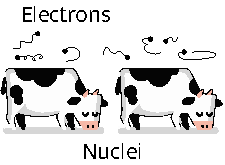
\includegraphics[width=1.75in]{img/born-oppenheimer-cow-fly.pdf}
}
\captionof{figure}{The fly/cow analogy of the Born--Oppenheimer approximation.}
}
The Hamiltonian then takes a simpler form
\begin{equation}
\hat{H}_\mathrm{BO} = \hat{T}_\mathrm{e} + \hat{V}_\mathrm{ee} + \hat{V}_\mathrm{en} + V_\mathrm{nn}
\end{equation}
The first term in this expression is just the kinetic energy of the electrons. The second term accounts for the electron-electron repulsion energy. The third term is the electron-nuclear attraction (attractive force acting on the electron). In this approximation, the last term is just a constant, which accounts for the nuclear-nuclear repulsion energy.\mnote{
The nuclear-nuclear repulsion energy is given by
\begin{equation}
V_\mathrm{nn} = \frac{1}{4\pi \epsilon_0}  \sum_{i < j}^{\mathrm{nuclei}} \frac{q_i q_j}{R_{ij}}
\end{equation}
}

The Born--Oppenheimer approximation is fundamental to our understanding of chemistry and  it one that you are already very familiar with, even though you might have not realized it.
This approximation is implicitly assumed when you first learn about quantum mechanics in introductory chemistry courses.
Once we solve the Schr\"{o}dinger equation in the BO approximation, we get an energy that depends on the coordinates of the nuclei
\begin{equation}
E = E(\mathbf{R}_1,  \mathbf{R}_2,\ldots)
\end{equation}
This is why we can talk about a molecule having a certain energy at a given nuclear configuration.
The quantity $E(\mathbf{R}_1,  \mathbf{R}_2,\ldots)$ represents the potential felt by the nuclei due to the interaction with the electrons, and since it is a function of many variables it is commonly called the \emph{potential energy surface}.


\section{Atomic units}
When doing computations on atoms or molecules it is convenient to use \emph{atomic units} (abbreviated a.u.), which are defined by the following conditions
\begin{align}
\text{electron mass} & = m_e = 1\\
\text{electron charge} & = e = 1\\
\text{action} & = \hbar = \frac{h}{2\pi} = 1\\
\text{Coulomb's constant} & = k_e = \frac{1}{4\pi \epsilon_0} = 1
\end{align}
These are natural units because the charge and mass of the particles we want to describe (electrons) are close to one.
In practice, it means that we will often avoid carrying around powers of ten in computations.

The following table shows the name and conversion factors between atomic units and SI units:
\begin{table}[htbp]
\centering
\begin{tabular}{lll}
\toprule
Dimension & Symbol (Name) & Value in Other Units\\
\midrule
Length & $a_0$ (bohr) & 0.52918 \AA{}  = $0.52918 \times 10^{-10}$ m\\ 
Mass & $m_e$ & $9.1095 \times 10^{-31}$ Kg \\
Charge & $e$ & $1.6022 \times 10^{-19}$ C \\
Action & $\hbar$ & $1.05457 \times 10^{-34}$ J $\cdot$ s \\
%Coulomb's constant & $\frac{1}{4\pi \epsilon_0}$ & $ \times 10^{-34}$ J $\cdot$ s \\
Energy & $E_{\rm h}$ (Hartree) & 627.51 kcal/mol \\
& & 27.211 eV \\
& & 219474.63 cm$^{-1}$ \\
& & $4.3598 \times 10^{-18}$ J\\
Time & & $2.41889 \times 10^{-17}$ s $\approx 1/41.3$ fs\\
\bottomrule
\end{tabular}
%\caption{Remember, \emph{never} use vertical lines in tables.}
\label{tab:atomicunits}
\end{table}

The speed of light in atomic units is $\alpha^{-1}\approx 137$ a.u.\mnote{The quantity $\alpha$ is also known as the fine-structure constant.}

\begin{aside}
\section*{Calculation or computation?}
What word should we use when we want to describe the result of some computational procedure used to determine the properties of molecule?
Often the words \emph{computation} and \emph{calculation} are used interchangeably, however, the word computation best conveys the meaning of the results of a mathematical calculation done with a computer. Here are dictionary definitions of these two terms:
\begin{quote}
Calculation: A mathematical determination of the size or number of something
\end{quote}
\begin{quote}
Computation: The action of mathematical calculation. The use of computers, especially as a subject of research or study.
\end{quote}
\end{aside}



\end{document}